% Oblici 2x1/1x2 nisu standardni šabloni paketa karnaugh-map.
% Indeksi vertikalnog primera namerno su 1,0 kao u originalu.
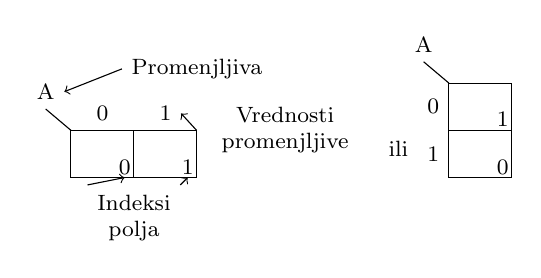
\begin{tikzpicture}[font=\fontsize{8}{9.5}\selectfont,x=8mm,y=6mm]
\draw (0,0) rectangle (2,1) (1,0)--(1,1);
\draw (0,1)--(-.4,1.45) node[above] (a) {A};
\node[above] at (.5,1) (v0) {0};\node[above] at (1.5,1) (v1) {1};
\node[anchor=south east,inner sep=1pt] at (1,0) (i0) {0};
\node[anchor=south east,inner sep=1pt] at (2,0) (i1) {1};
\node at (2.0,2.3) (prom) {Promenjljiva};
\draw[->] (prom.west)--(a.east);
\node[align=center,text width=20mm] at (3.4,1.0) (val) {Vrednosti\\promenjljive};
\draw[->] (val.west)--(v1.east);
\node[align=center] at (1,-.85) (ind) {Indeksi\\polja};
\draw[->] (ind.north west)--(i0.south);
\draw[->] (ind.north east)--(i1.south);
\node at (5.2,.6) {ili};
\draw (6,0) rectangle (7,2) (6,1)--(7,1);
\draw (6,2)--(5.6,2.45) node[above] {A};
\node[left] at (6,1.5) {0};\node[left] at (6,.5) {1};
\node[anchor=south east,inner sep=1pt] at (7,1) {1};
\node[anchor=south east,inner sep=1pt] at (7,0) {0};
\end{tikzpicture}
